\section{Auswertung}
\label{sec:auswertung}
\subsection{invariante Masse der B-Mesonen in simulierten Daten}

Zu Beginn werden die \texttt{\.root}-Dateien der simulierten Daten eingelesen die Features betrachtet.
Das Ziel im ersten Teil ist, die invariante Masse der B-Mesonen zu bestimmen. Da dies nicht direkt funktioniert, muss dies \"uber die Tochterteilchen getan werden.
Betrachten wird ausschie\ss lich der Zerfall
\begin{equation}
  B^{\pm} \to \symup{K}^{\pm} \symup{K}^{+} \symup{K}^{-}\,.
\end{equation}
Um die invariante Masse zu bestimmen wird die Beziehung aus der speziellen Relativit\"atstheorie
\begin{equation}
  \symup{E}^2 = \symup{p}^2 + \symup{m}^2\,,
  \label{eqn:relativityEQ}
\end{equation}
verwendet, welche Energie, Masse und Impuls verkn\"upft.

Aus den Daten werden die Dreierimpulse der Tochterteilchen entnommen.
Diese werden zunächst in einem Diagramm dargestellt um diese zu überprüfen.

\begin{figure}[!htb]
  \centering
  \minipage[c]{0.32\textwidth}
    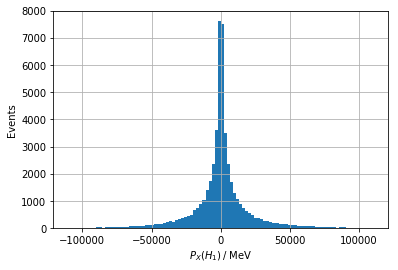
\includegraphics[width=\linewidth]{plots/sim_px_kaon1.png}
    \label{fig:px}
  \endminipage\hfill
  \minipage[c]{0.32\textwidth}
    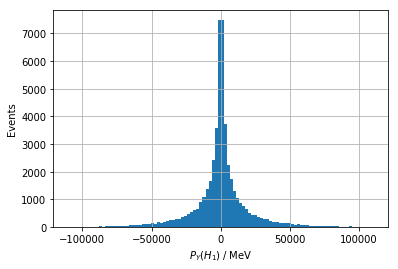
\includegraphics[width=\linewidth]{plots/sim_py_kaon1.png}
    \label{fig:py}
  \endminipage\hfill
  \minipage[c]{0.32\textwidth}
    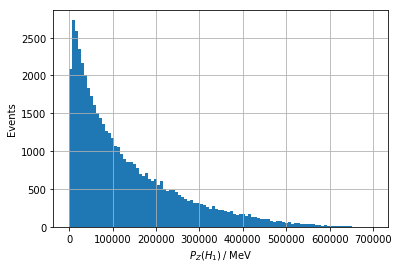
\includegraphics[width=\linewidth]{plots/sim_pz_kaon1.png}
    \label{fig:pz}
  \endminipage
  \caption{Die Impulse in x, y und z Richtung von Kaon1.}
  \label{fig:momenta}
\end{figure}

Es ist in Abbildung \ref{fig:momenta} zu erkennen, dass die Teilchen stark in z-Richtung geboostet sind, was auch zu erwarten ist bei B-Mesonen.

Um die invariante Masse zu berechnen, wird zun\"achst die Energie der B-Mesonen bestimmt.
\begin{equation}
  \symup{E}(B^{\pm}) =
  \sqrt{\left(\sum_{i = 1}^{3} \vec{\symup{p}}_i\right)^2 + \left(\sum_{i = 1}^{3} \symup{m}_i\right)^2}
\end{equation}

F\"ur die Massen wird die Massenhypothese der Kaonen eingesetzt, da dies der interessante Endzustand ist.

Mit der berechneten Energie kann durch umstellen von Gleichung \eqref{eqn:relativityEQ} auf den Impuls und damit auch auf das Betragsquadrat der B-Mesonen geschlossen werden.

In Abbildung \ref{fig:invMassB} liegt der Massenpeak bei etwa $\SI{5279.2}{\mega\electronvolt}$, was sehr eng an dem Wert des PDG liegt.
%Hier müssen wir noch eine Quelle zur PDG Masse einfügen
Dieser Peak ist so scharf, da es sich hier im simulierte Daten handelt. In Wirklichkeit sollte der Peak breiter gefächert sein.

\begin{figure}[!htb]
  \centering
  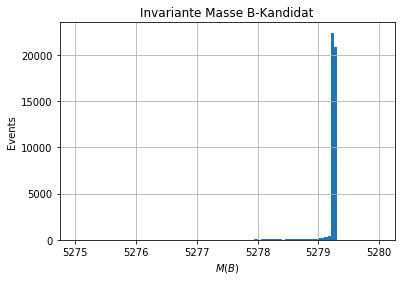
\includegraphics[width=0.8\textwidth]{plots/sim_inv_masse_B.png}
  \caption{Invariante B Masse in den simulierten Daten.}
  \label{fig:invMassB}
\end{figure}

\subsection{invariante Masse der B-Mesonen in echten Daten}
Als n\"achstes wird die invariante Masse der echten B-Mesonen rekonstruiert.
Hierzu wird zun\"achst eine Vorselektion durchgef\"uhrt um den oben genannten Endzustand zu verwenden.
Dazu verwenden die folgenden Schnitte.
\begin{enumerate}
  \item \texttt{H1\_isMuon} == False
  \item \texttt{H1\_ProbPi} < 0.5
  \item \texttt{H1\_ProbK} > 0.5
\end{enumerate}

Diese Schnitte werden analog auch f\"ur Tochterteilchen 2 und 3 angewandt.
Die Verteilungen der Wahrscheinlichkeiten ob ein Endzustandsteilchen ein Kaon oder Pion ist werden geplottet um die Schnitte auf \texttt{H1\_ProbK} und \texttt{H1\_ProbPi} sch\"arfer zu machen falls nötig.
Dies hat zur Folge, dass sehr viel Statistik Im Signal verloren geht und noch ziemlich viel Hintergrund vorhanden ist. Deswegen werden die Schnitte wie oben belassen.
Die Wahrscheinlichkeitsverteilungen mit unserem hypothetischen Schnitt ist in Abbildung \ref{fig:probCuts} zusehen.

\begin{figure}[!htb]
  \centering
  \minipage[c]{0.48\textwidth}
    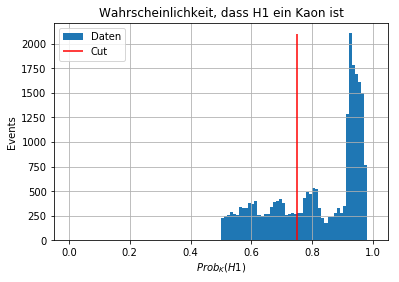
\includegraphics[width=\linewidth]{plots/probability_kaon1.png}
    \label{fig:probK}
  \endminipage\hfill
  \minipage[c]{0.48\textwidth}
    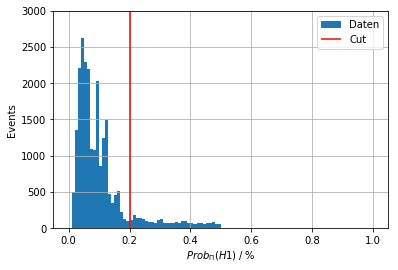
\includegraphics[width=\linewidth]{plots/probability_pion1.png}
    \label{fig:probPi}
  \endminipage
  \caption{Wahrscheinlichkeitsverteilungen f\"ur Kaon und Pion.}
  \label{fig:probCuts}
\end{figure}

Anschlie\ss end wird, wie schon bei den simulierten Daten, die invariante Masse der B-Mesonen berechnet. Diese ist in Abbildung \ref{fig:realBMass} dargestellt.

\begin{figure}[htb]
  \centering
  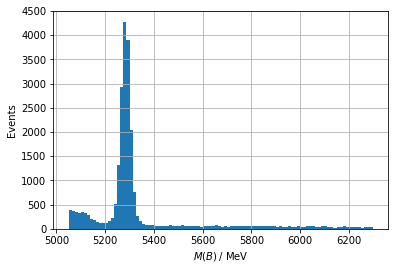
\includegraphics[width=0.8\textwidth]{plots/real_data_inv_masse_B.png}
  \caption{Invariante B Masse in den echten Daten.}
  \label{fig:realBMass}
\end{figure}
\newpage
\subsection{globale CP-Asymmetrie}
Um den Materie-Antimaterie Unterschied sichtbar zu machen, m\"ussen $B^{-}$ von den $B^{+}$-Mesonen separieren werden.
Hierzu haben wir die Ladungen der Tochterteilchen multipliziert.
Ist das Produkt $+1$,wird das Ereignis zu den $B^{-}$ gez\"ahlt, andernfalls zu den $B^{+}$.
Das bedeutet der Asymmetriefaktor berechnet sich gem\"a\ss
\begin{equation}
  \symup{A} = \frac{N^{+} - N^{-}}{N^{+} + N^{-}} = 0.\overline{037}
\end{equation}

Daraus berechnet sich die statistische Unsicherheit und die Signifikanz mittels
\begin{align}
  \sigma_A &= \sqrt{\frac{1 - A^2}{N^{+} + N^{-}} } \approx 0.006 \\
  \text{Signifikanz} &= \frac{\symup{A}}{\sigma_A} \approx 5.729
\end{align}

Ohne Ber\"ucksichtigung der systematischen Unsicherheiten gilt dies als Entdeckung der CP-Asymmetrie.
Da es jedoch eine Produktionsassymetrie von Materie zu Antimaterie von circa $\SI{1}{\percent}$ gibt, wird dies f\"ur die gesamte Unsicherheit mit berechnet.
\begin{equation}
  \text{Sig}_{ges} = \frac{\symup{A}}{\sqrt{\sigma_A^2 + 0.01^2}} \approx 3.11
\end{equation}

Da dieser Wert kleiner als 5$\sigma$ und gr\"o\ss er als 3$\sigma$ ist, gilt die berechnte CP-Asymmetrie nur als Hinweis darauf.

\subsection{Zweik\"orper-Resonanzen f\"ur simulierte Daten}
Naiv betrachtet ist der B-Meson Zerfall in drei Kaonen ein Dreik\"orperzerfall, doch es kann auch passieren, dass zun\"achst eine neutral geladene Zwischenresonanz erzeugt wird, welche wiederum in zwei Kaonen zerf\"allt.
Um diese Zwischenresonanzen herauszufiltern werden Dalitz Plots verwendet, da diese Resonanzen als B\"ander sichtbar machen und so leicht identifiziert werden k\"onnen.

Die Kinematik eines Dreik\"orperzerfalls wird eindeutig durch zwei unabh\"angige Variablen ausgedr\"uckt. Hierbei wird die invariante Masse von jeweils zwei der drei Endzustandsteilchen verwendet.
Das bedeutet es gibt drei m\"ogliche Kombinationen:
$M_{1,2}$, $M_{2,3}$, $M_{1,3}$.
Bevor jedoch zwei der Kombinatione ausgew\"ahlt werden k\"onnen, muss die Ladung jedes Tochterteilchens identifiziert worden sein.
Denn die Resonanz muss neutral geladen sein. da aber zwei der drei Teilchen die selbe Ladung besitzen, beispielsweise Teilchen 1 und Teilchen 2, darf $M_{1,2}$ nicht als Variable verwendet werden.
Eine doppelt geladene Resonanz ist au\ss erdem f\"ur Mesonen verboten, da diese immer aus einem Teilchen und einem Antiteilchen bestehen.

In Abbildung \ref{fig:m12} und \ref{fig:m13} sind die Resonanzen f\"ur die Kombinationen $M_{1,2}$ und $M_{1,3}$ dargestellt.

\begin{figure}[htb]
  \centering
  \minipage[c]{0.48\textwidth}
    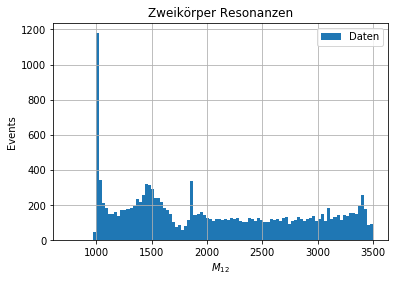
\includegraphics[width=\linewidth]{plots/real_data_twobody_resonance_m12.png}
    \caption{Ungeladene Resonanz $M_{1,2}$.\label{fig:m12}}
  \endminipage\hfill
  \minipage[c]{0.48\textwidth}
    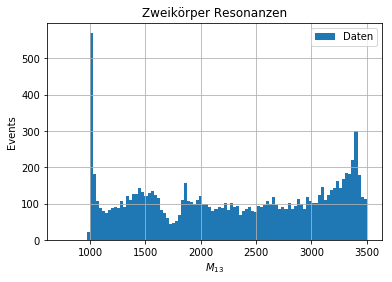
\includegraphics[width=\linewidth]{plots/real_data_twobody_resonance_m13.png}
    \caption{Ungeladene Resonanz $M_{1,3}$.\label{fig:m13}}
  \endminipage
  \label{fig:resonances}
\end{figure}

Die quadrierten Massen ergeben aufgetragen gegeneinander den Dalitz Plot, welcher in Abbildung \ref{fig:dalitzSim} zusehen ist.

\begin{figure}[htb]
  \centering
  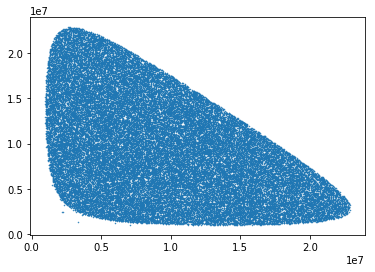
\includegraphics[width=0.8\textwidth]{plots/sim_dalitz_plot_m12_m13.png}
  \caption{Dalitz PLot f\"ur simulierte Daten.}
  \label{fig:dalitzSim}
\end{figure}

Der Dalitz Plot ist kontinuierlich mit Daenpunkten ausgef\"ullt und es sind keine B\"ander erkennbar. Das liegt daran, dass in den simulierten Daten keine Resonanzen vorhanden sind.
